\chapter{Le Grand collisionneur de hadrons (LHC)}
\renewcommand\chapterillustration{LHC/lhc}
\ThisULCornerWallPaper{1}{\chapterillustration}
\minitoc
\vspace{1cm}
\lettrines{C}{e} chapitre décrit le complexe des accélérateurs du CERN\footnote{Organisation Européenne pour le Recherche Nucléaire} qui permet d'accélérer les particules, afin d'avoir un faisceau de particule avec une énergie suffisante pour être injecter dans le Grand collisionneur de hadrons (LHC\footnote{Large Hadron Collider}) est atteindre une énergie final de ($7$ TeV). Cette déscription bien que succinte est nécessaire car de nombreux résultats obtenus durant cette thèse ont nécessité l'utilisation d'accélérateur de ce complexe. Une description du LHC est également donnée, car ses performances présentes et futurs déterminent les choix technologiques des détecteurs utilisant son faisceau.

\section{Le complexe d'accélérateurs du CERN}

Le complexe d'accélérateur (\ref{complexe}) du CERN est une série de machines qui délivrent des faisceaux de particules d'énergies de plus en plus élevés. Chaque machine accélère les faisceaux et les injecte dans la machine suivante. Le dernier accélérateur du complexe est le Large Hadron Collider.

Le programme du LHC est surtout basé sur des collisions prontons-protons. Cependant chaque année, environ un mois est consacré ou collision d'ions lourds (plomb-plomb) ou (proton-plomb) afin d'étudié notamment le plasma de quarks et gluons l'une des phases de l'Univers peu après le Big Bang. 

Dans le cas de ces collisions, la chaine d'accélération est constituée du Linear Accelerator 3 (LINAC 3), du Low Energy Ion Ring (LEIR) utilisé pour le stockage des ions et leur refroidissement. La chaine d'accélération est ensuite identique à celle pour les collisions proton-proton.

\begin{minipagewithmarginpars}[h]{\textwidth}
  	\centering
	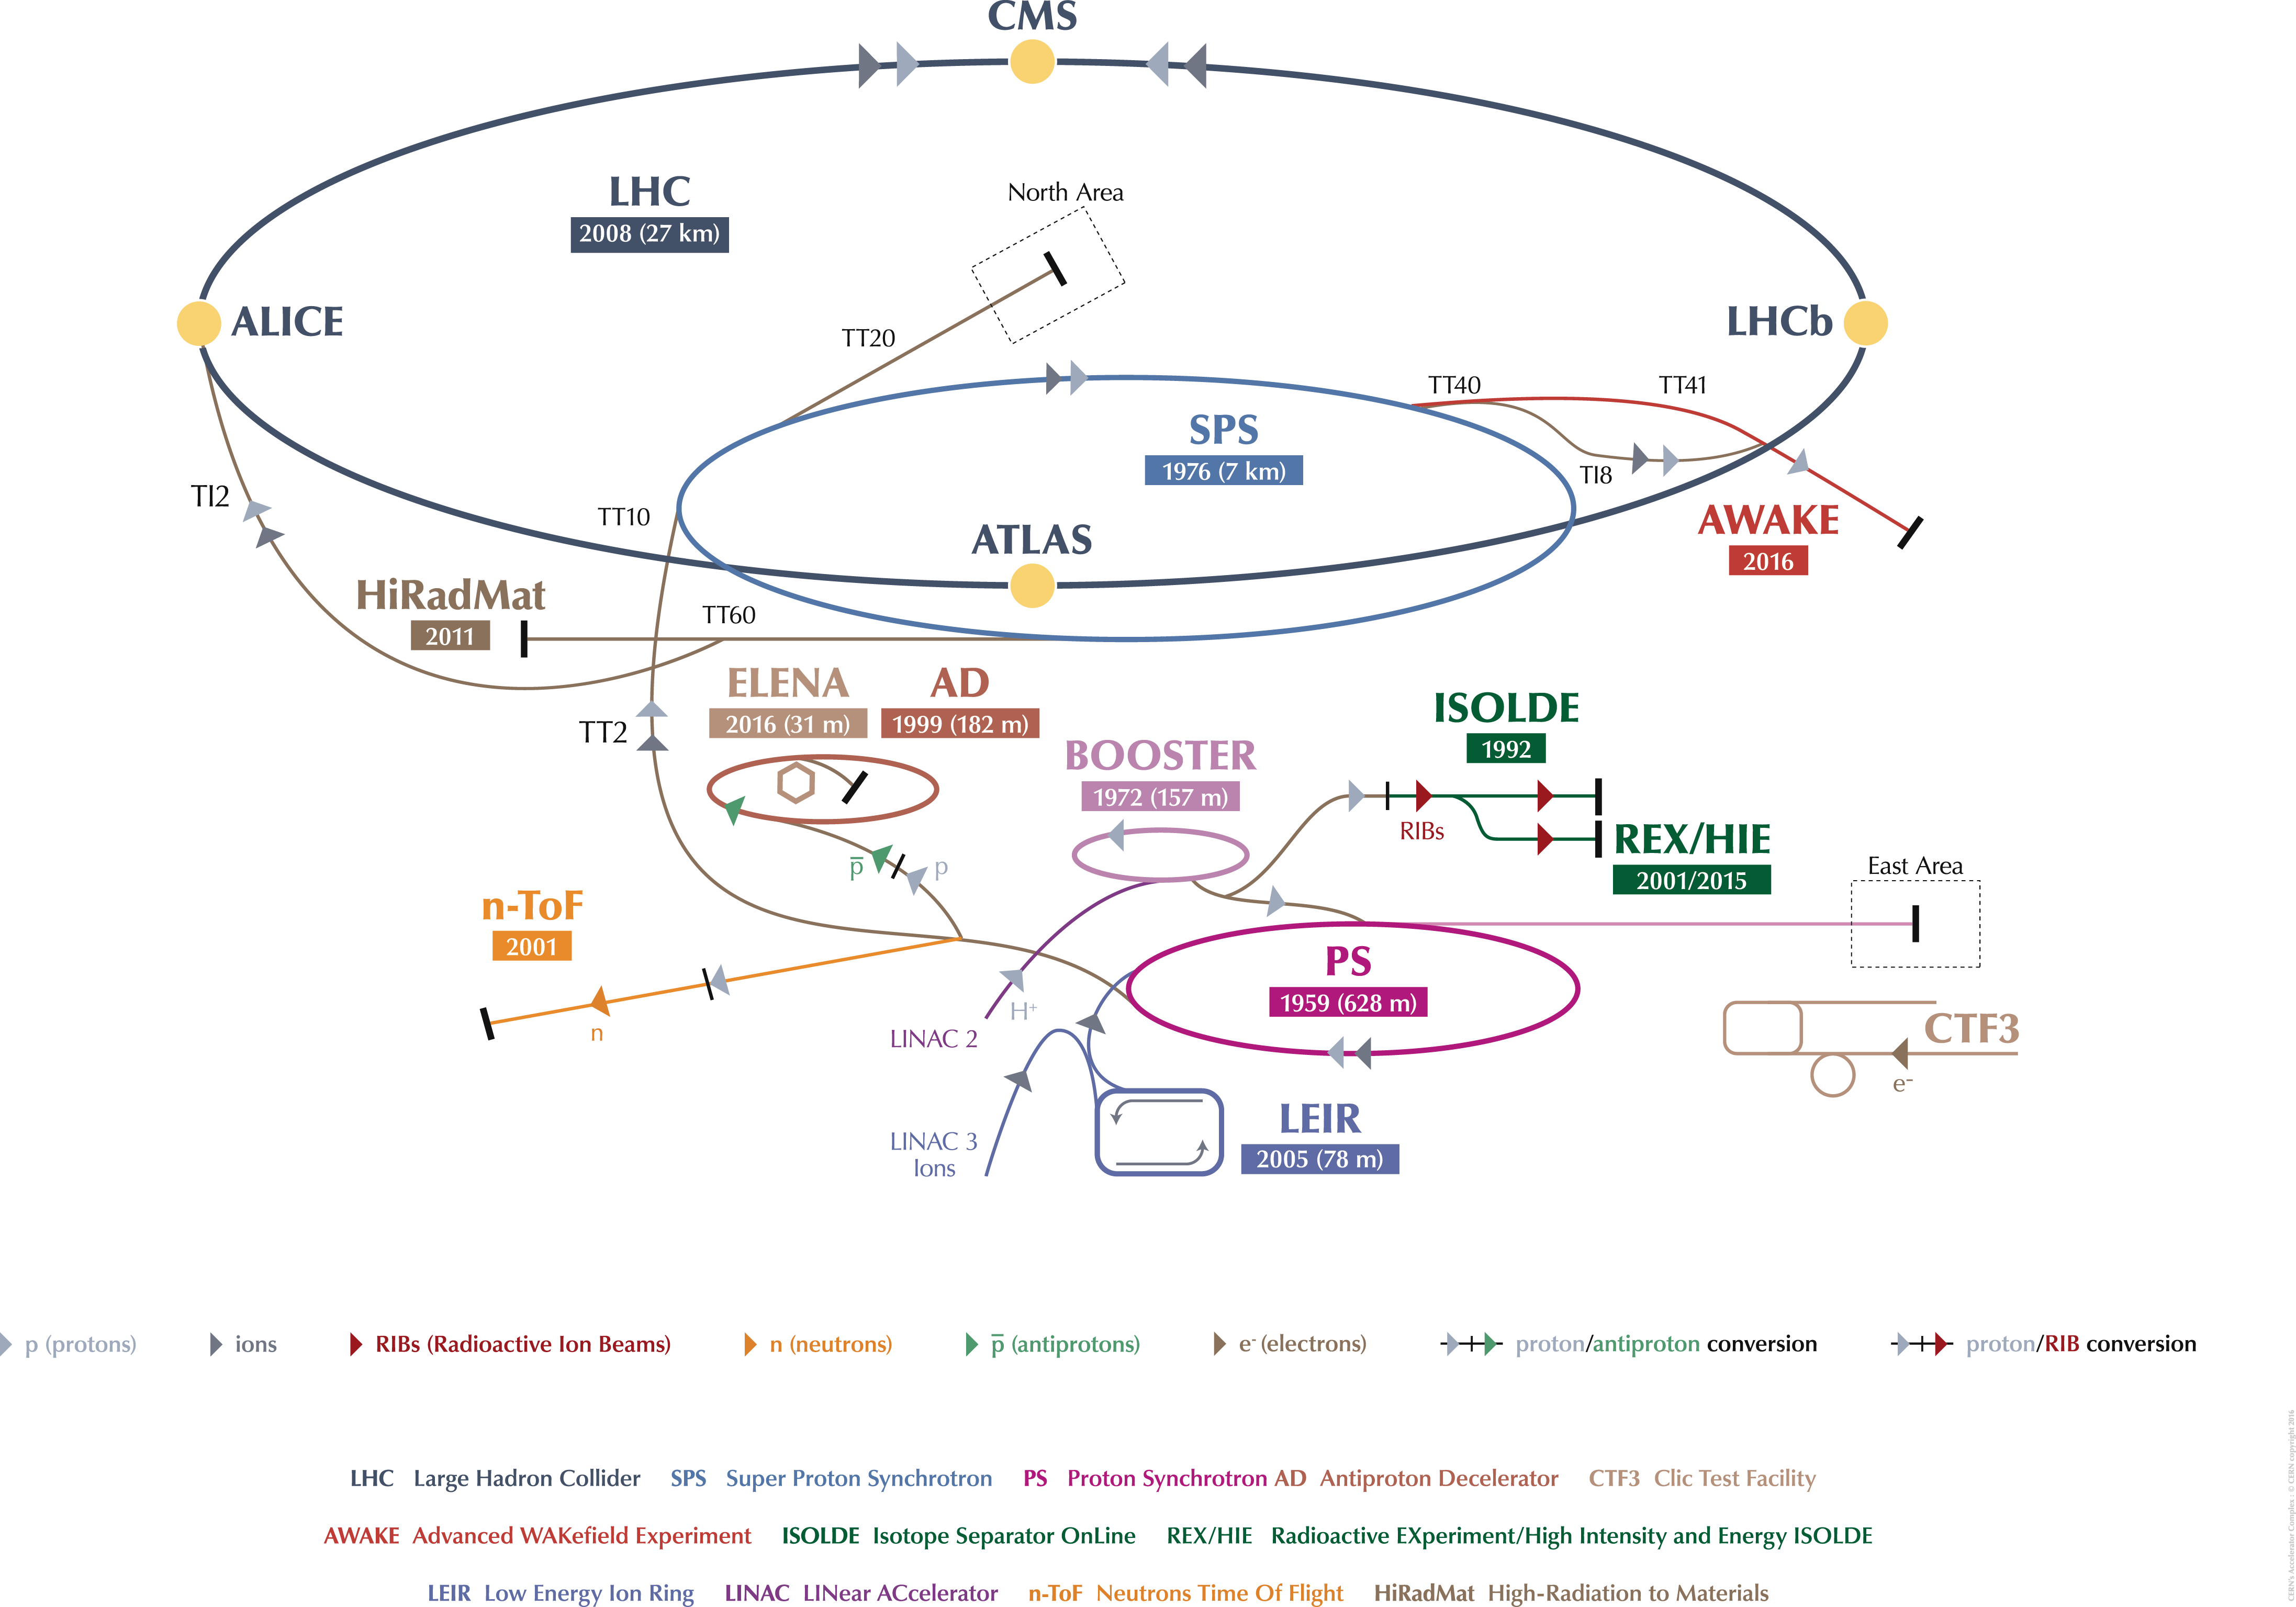
\includegraphics[scale=0.25]{LHC/complexe.png}
  	\captionof{figure}{Schéma du complexe d'accélération du CERN. La chaine d'injection du LHC est constituée du Linac 2, du Booster, du PS et du SPS}
  	\label{complexe}
  	\par 	
\marginpar
{
	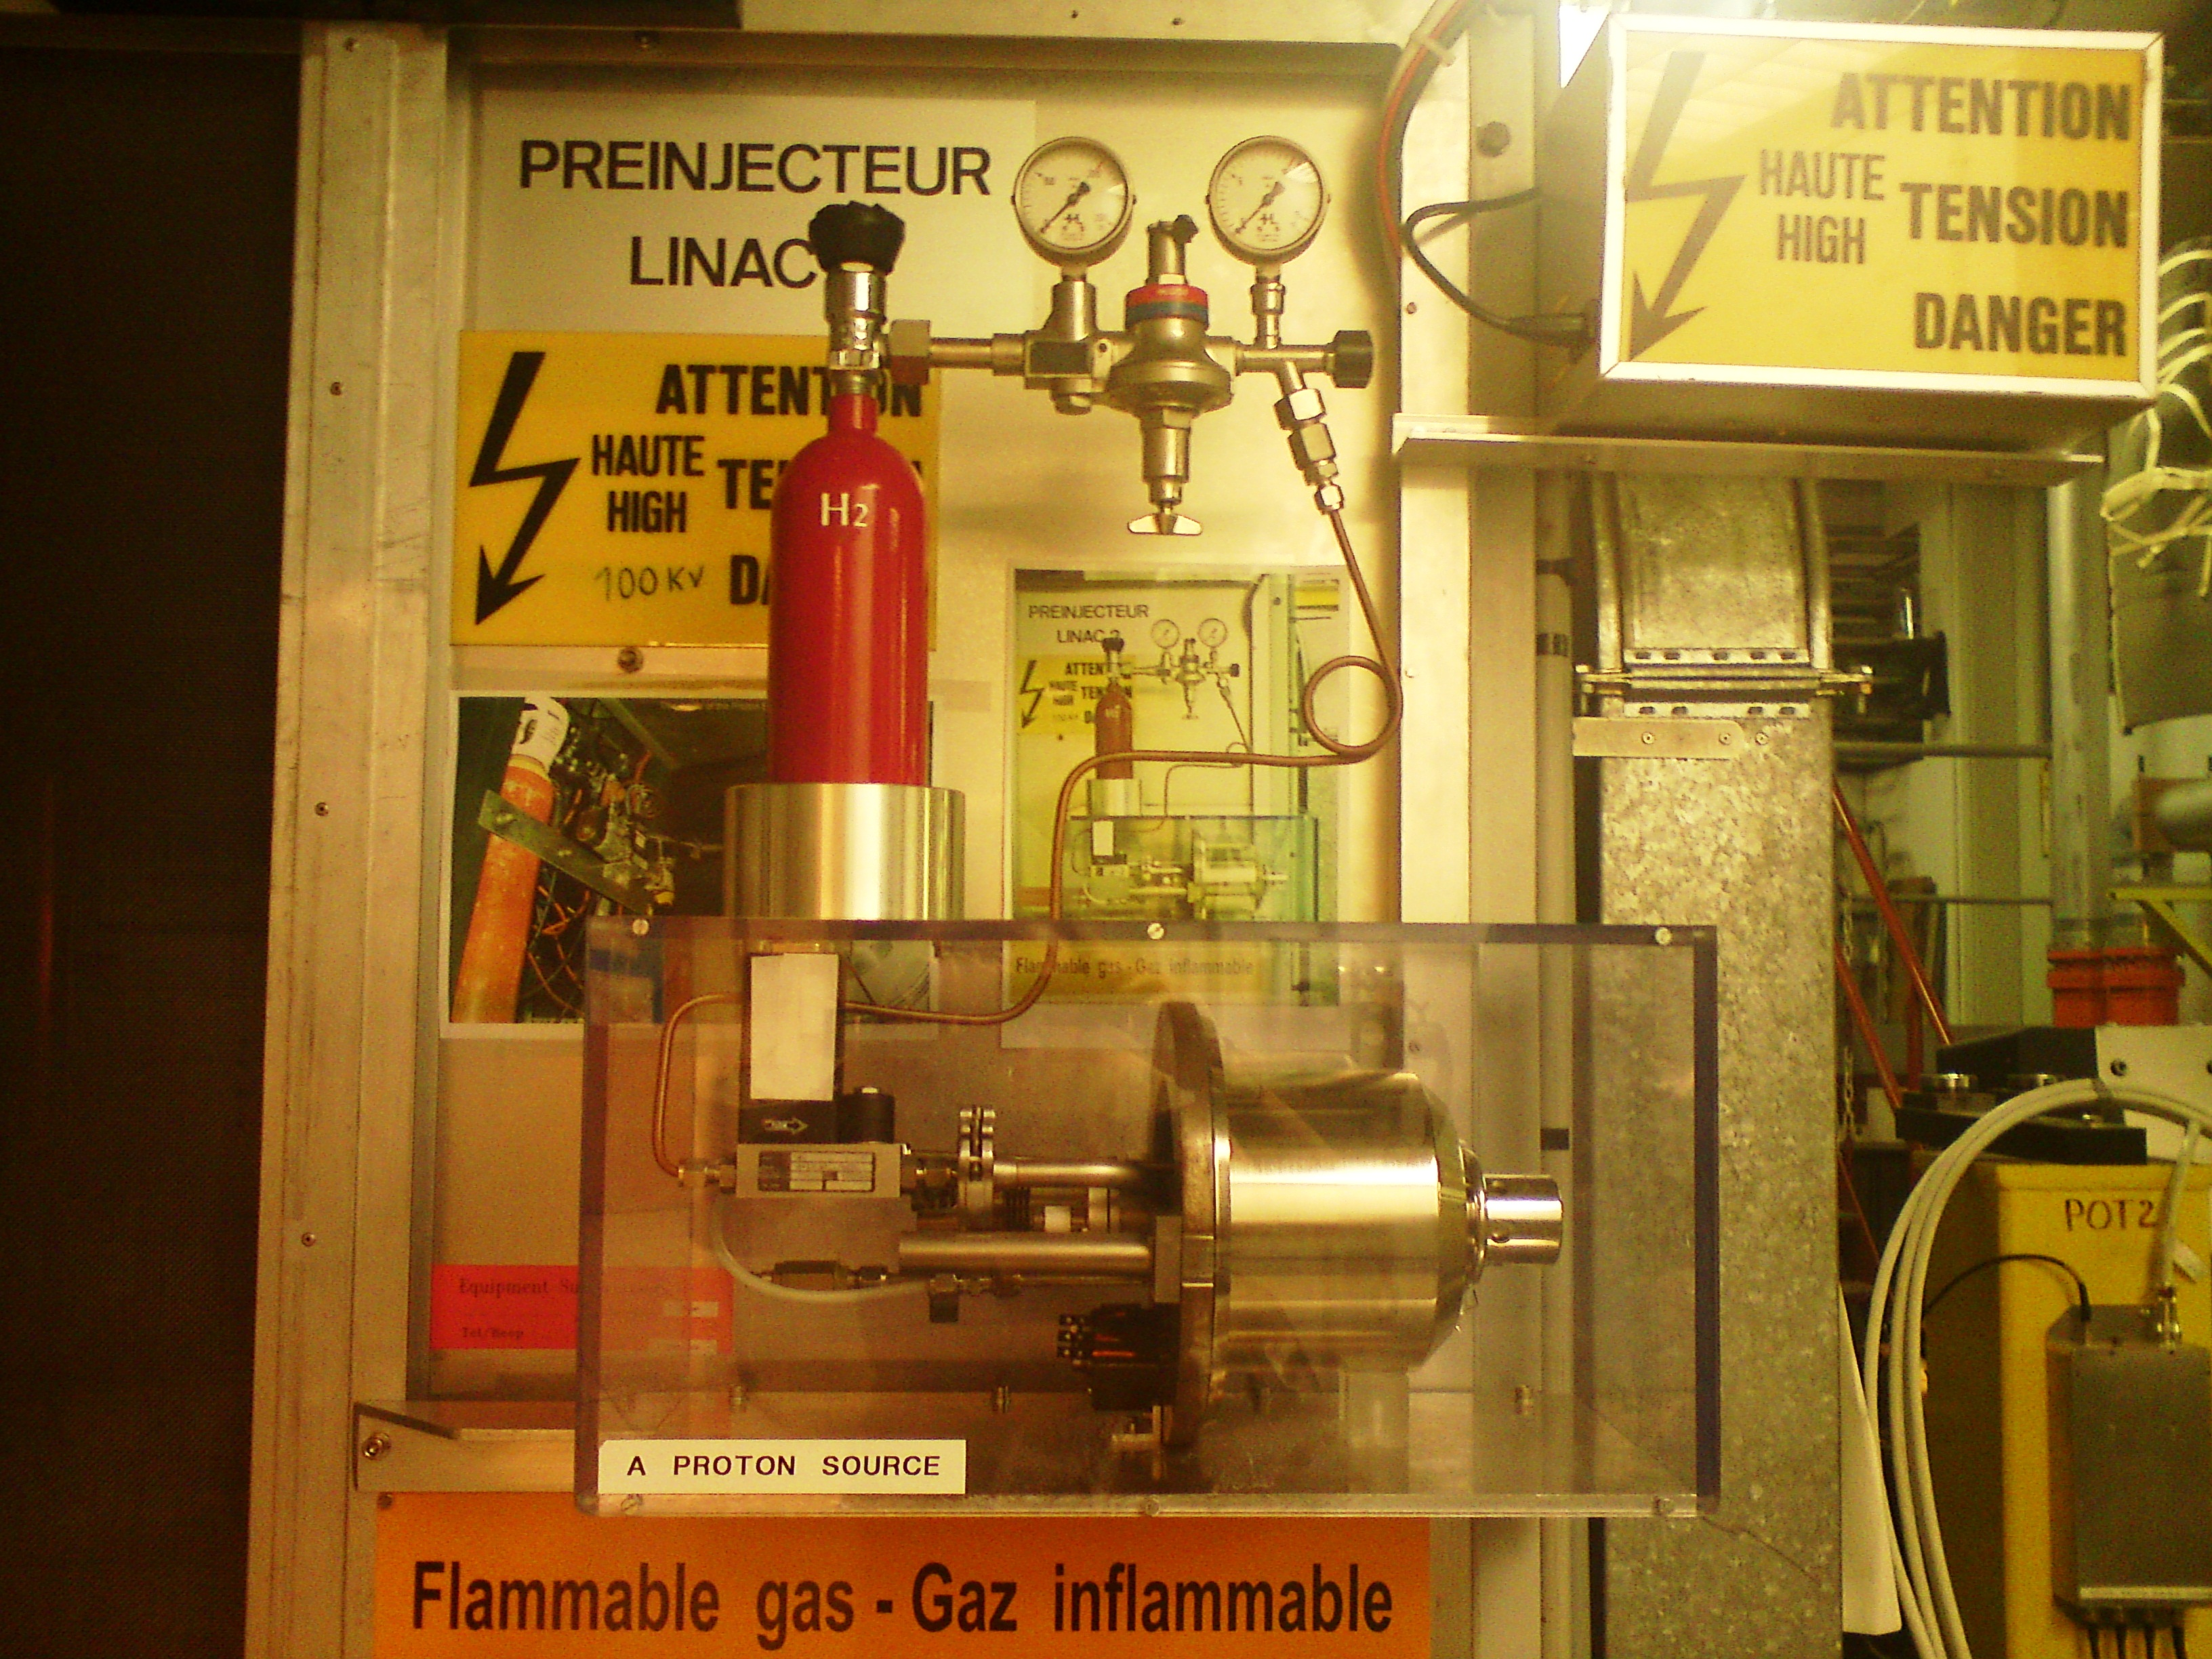
\includegraphics[width=\marginparwidth]{LHC/Bouteille.jpg}
	\label{bouteille}
    	\captionof{figure}{Source des protons du LHC.}
}	
\end{minipagewithmarginpars}

\marginpar
{
	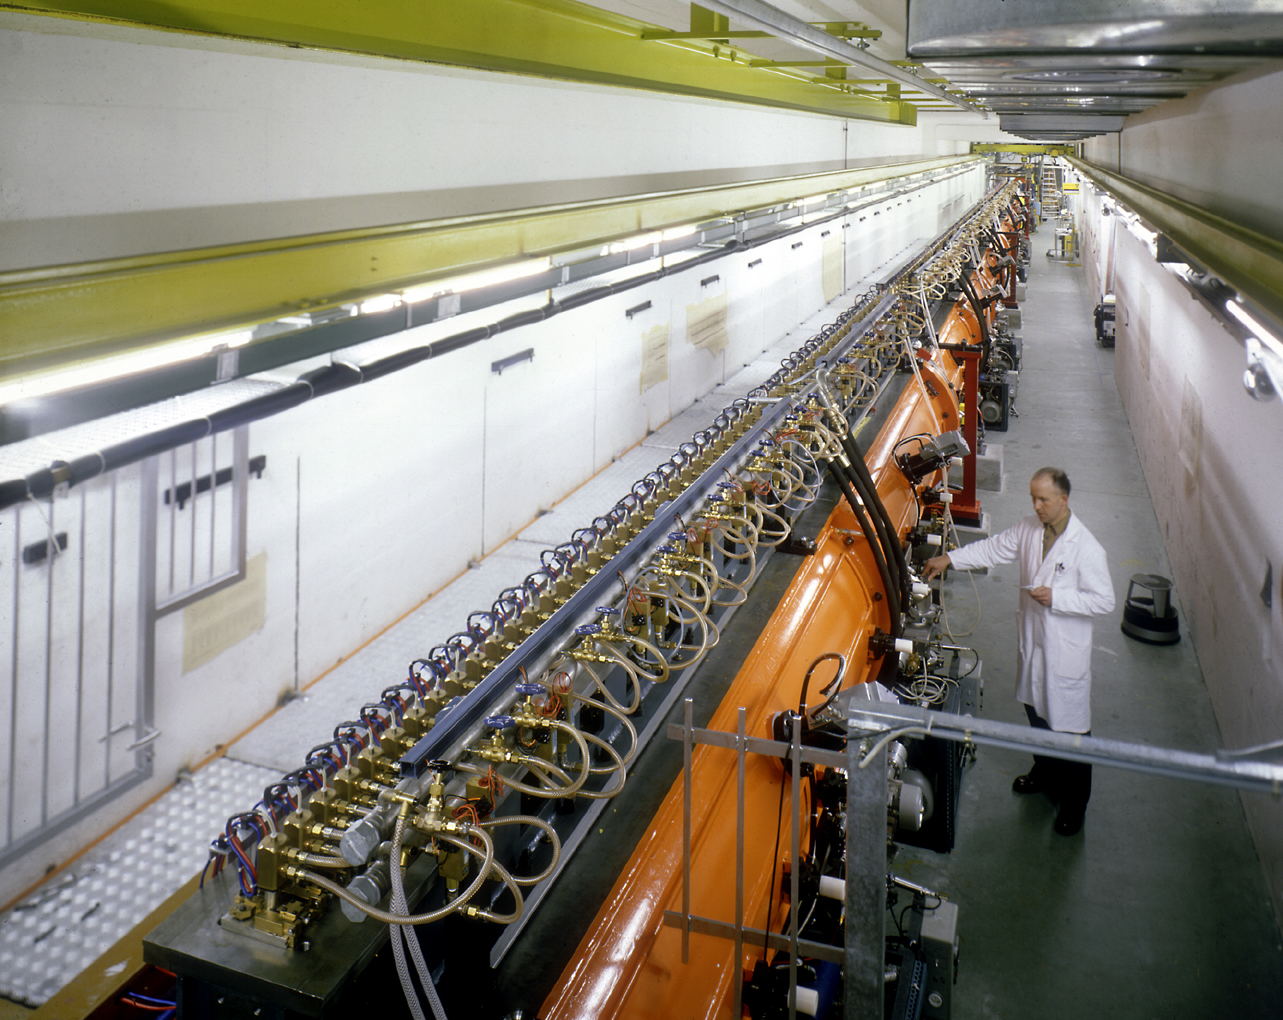
\includegraphics[width=\marginparwidth]{LHC/linac2.jpg}
    \captionof{figure}{Photo du LINAC 2.}
    	\label{linac2}
}

\marginpar
{
	
	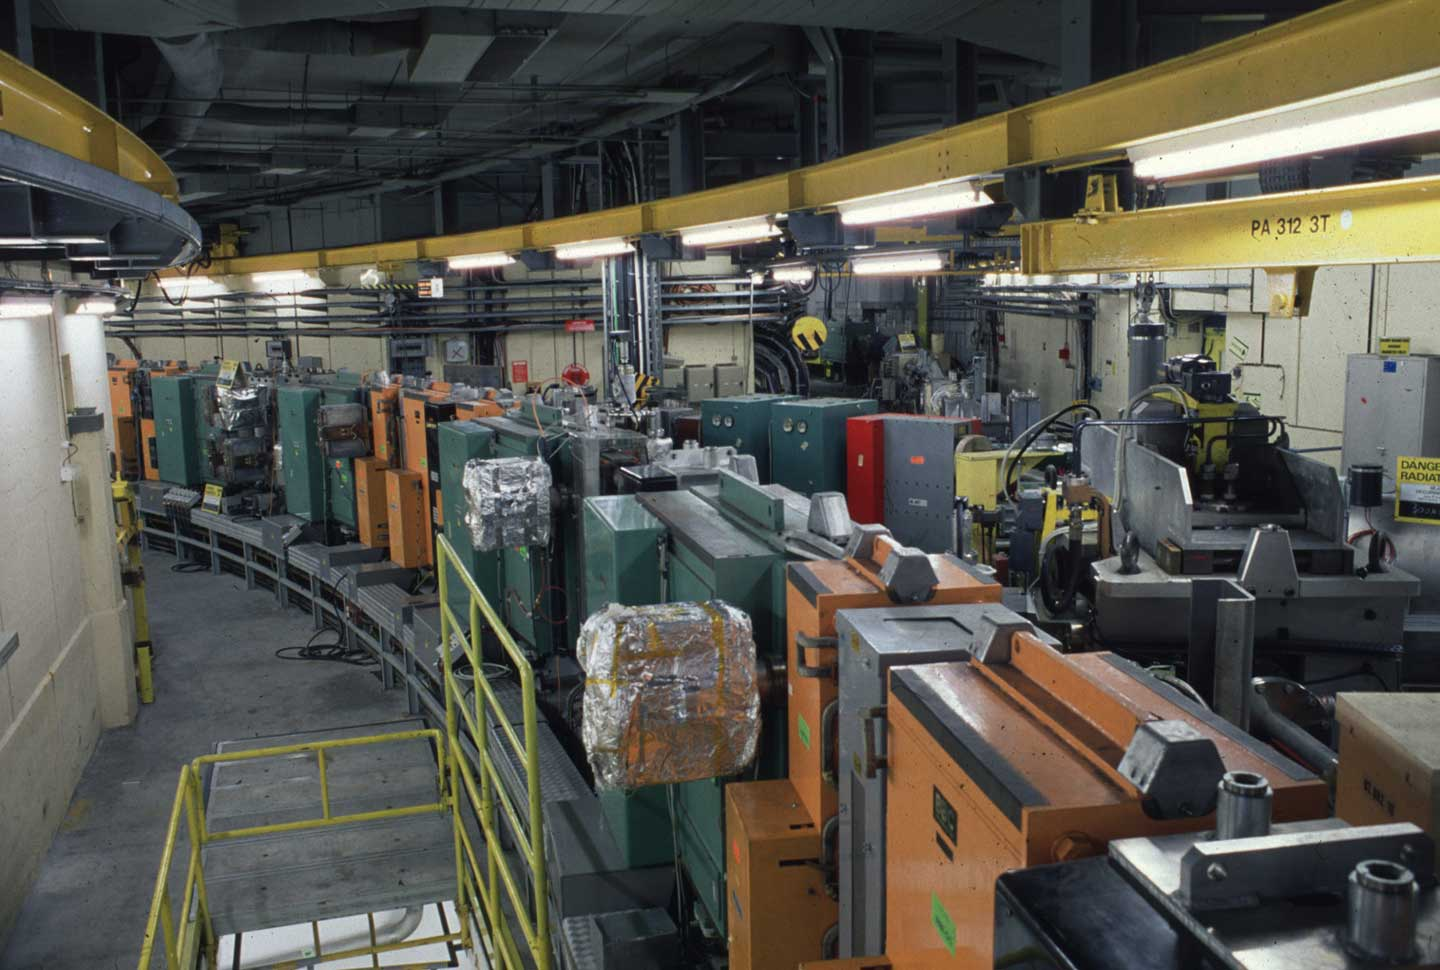
\includegraphics[width=\marginparwidth]{LHC/booster.jpg}
    \captionof{figure}{Photo du Booster du Synchrotron à protons.}
    	\label{booster}
}

\marginpar
{
	
	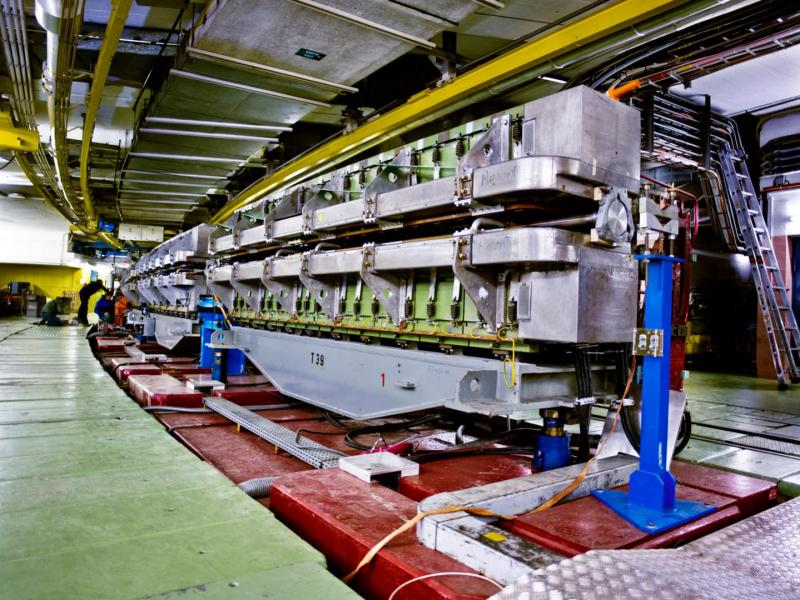
\includegraphics[width=\marginparwidth]{LHC/ps.jpg}
    \captionof{figure}{Photo du PS.}
    	\label{ps}
}

\marginpar
{
	
	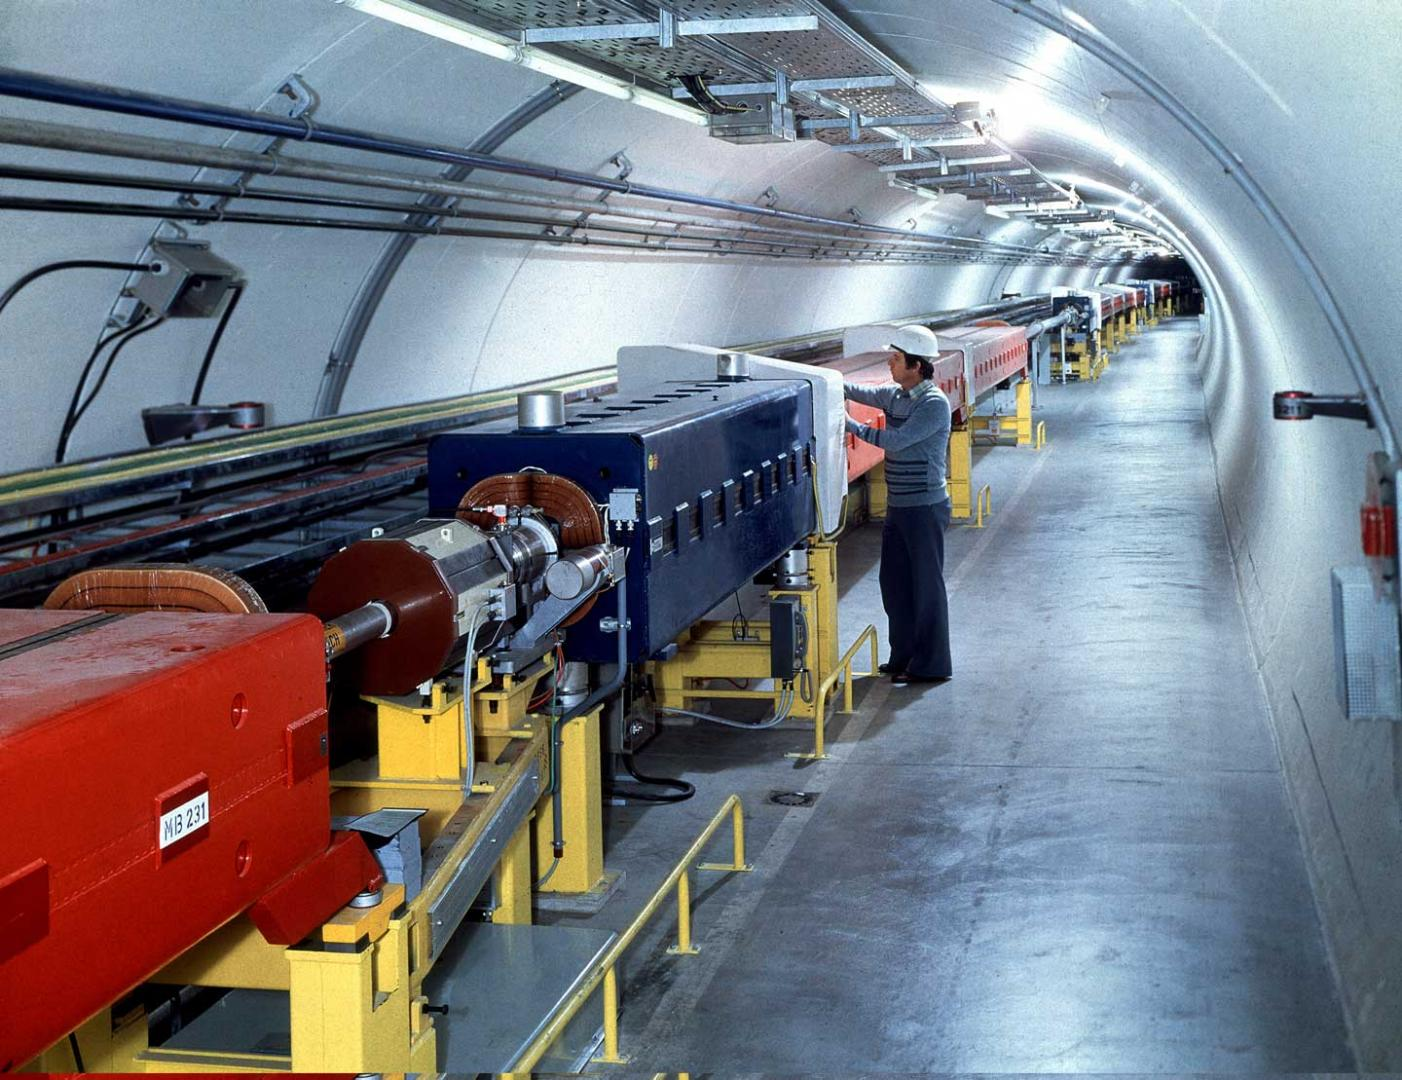
\includegraphics[width=\marginparwidth]{LHC/sps.jpg}
    \captionof{figure}{Photo du SPS.}
    	\label{sps}
}
Pour les collisions proton-proton, la source de protons est une bouteille de dihydrogène gazeux (fig. \ref{bouteille}). Les atomes d’hydrogène sont soumis à un champ électrique, qui arrache leurs électrons et les ionises en $H^{+}$ (proton). Les protons extraits sont ensuite envoyés dans l'accélérateur linaire (LINAC 2 (fig. \ref{linac2})) ou ils atteignent l'énergie de 50MeV et sont $5\%$ plus massifs. Ils passe ensuite dans les 4 anneaux de 157m de circonférence du Booster du Synchrotron à protons (BOOSTER (fig. \ref{booster})) qui les amènent à une énergie de 1.4 TeV avant de les Injecté dans l'accélérateur suivant, le Synchrotron à protons (PS (fig. \ref{ps})). Cet accélérateur circulaire de 628 mètres de circonférence, permet aux faisceau d'atteindre une énergie de 25GeV; Il sert aussi à préparer le faisceau en le découpant en série de paquets (bunchs) de particules nécessaire au LHC. Ces bunchs sont ensuite envoyé dans le le supersynchrotron à protons (SPS (fig. \ref{sps})) d'une circonférence de 7km, ou l'énergie du faisceau atteint 450GeV. Les paquets sont regroupés pour formés des trains de paquets avant d'être enfin envoyé dans le Grand collisionneur de protons (LHC). L'injection et le guidage de faisceaux de tel énergie par des aimants supraconducteur rapide est une tâche délicate et pourrait détériorer l'accélérateur. Un faisceau de test de faible intensité "pilot beam" est donc injecter afin de mesurer et vérifier les paramètres. Le faisceau de haute énergie est ensuite séparer en deux et injecter dans deux conduits différents, l'un circulant dans un sens et l'autre dans le sens contraire. Ces faisceaux sont ensuite accélérer jusqu'à une énergie de 7TeV et ne se croisent qu'aux points d'intéractions.

\section{Le Large Hadron Collider}
LeLHC est le dernier accélérateur circulaire du complexe d'accélération. Il utilise le tunnel de 27km de circonférence situé à une centaine de mètres sous terre. Il fût construit pour acceuillir le Grand collisionneur électron-positron (LEP\footnote{Large Electron Positron collider}), qui fût en service de 1989 à 2000. Le LHC à été mit en service en 2008 est à été construit afin de produire de l'ordre de 600 millions de collisions proton-proton par seconde à une énergie au centre de masse de $\sqrt{s}=14 TeV$. Il est actuellement l'accélérateur de proton-proton le plus puissant du monde, et à permit de mettre en évidence l'existence du boson de Higgs, dernière pièce manquante du Modèle Standard.

Le LHC est un collissioneur de particules non fondamentales (hadrons) à l'inverse de son prédécesseur, le LEP qui utilisé des électrons et des positrons. Lors d'une collission entre hadrons, ceux sont ses constituant élementaires, les quarks et les gluons qui collissionnent entre eux. Ceux-ci possèdent seulement une portion de l'énergie du hadrons qui les contient. L'énergie du centre de masse de cette collision n'est donc pas connue avec précision. Le LHC est donc une machine de découverte de particules plutôt qu'une machine de mesures de précisions comme l'était le LEP, car il permet d'acceder à un large spectre en énergie. Généralement, les mesures de précision sont effectué grâce à des collisionneur utilisant des particules élémentaires ($e^{-}$,$e^{+}$); ils sont dans ce cas souvent linéaire afin d'éviter la perte d'énergie par rayonnement synchroton.

La figure (\ref{lhcschema}) est une vue schématique du LHC. En vérité le LHC n'est pas parfaitement circulaire, mais est composé de $8$ octants composés d'une section droite de longueur $~5$km est d'un secteur courbe d'une longueur de $~3$km (fig. \ref{octants}). Les sections droites sont utilisées afin de faire collisionner les deux faisceaux de protons venant en sens inverse l'un de l'autre. Il existe $8$ points d'interactions (P), mais seulement $4$ possèdent des détecteurs qui analyse les données issus de ces collisions : le point P1 pour ATLAS\footnote{A Toroidal LHC ApparatuS, détecteur généraliste.}, le point P2 pour ALICE\footnote{A Large Ion Collider Experiment, dédié au l'étude du plasma de quarks et gluons.}, le point P5 pour CMS\footnote{Compact Muon Solenoid, détecteur généraliste.} et le point P8 pour LHCb\footnote{Large Hadron Collider beauty experiment, dédié au quark b}.

\begin{minipagewithmarginpars}[h]{\textwidth}
  	\centering
	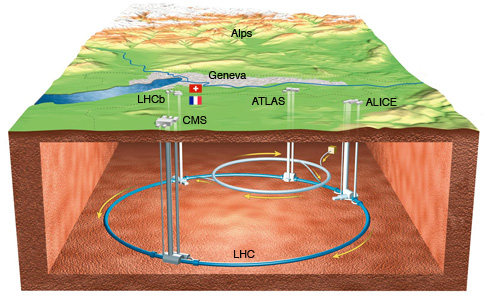
\includegraphics[scale=0.6]{LHC/CERNMap.jpg}
  	\captionof{figure}{Vue schématique du LHC.}
  	\label{lhcschema}
  	\par 	
\marginpar
{
	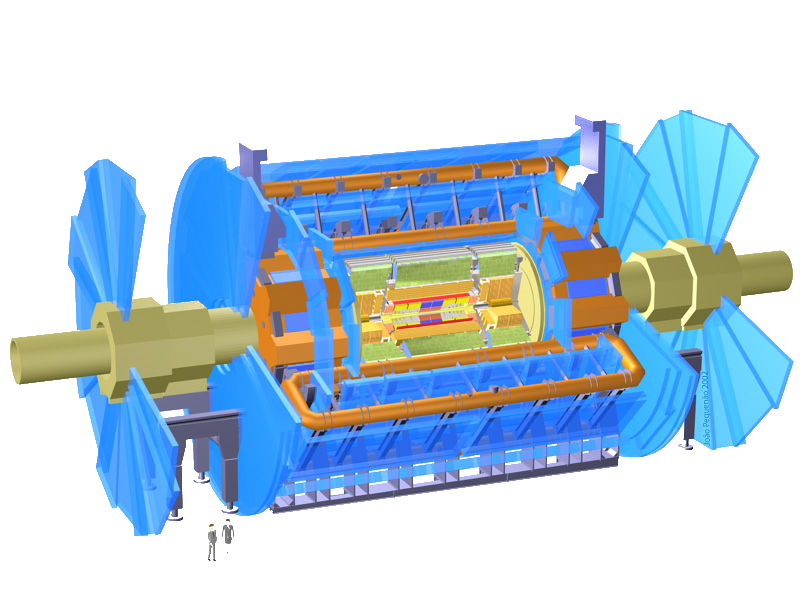
\includegraphics[width=\marginparwidth]{LHC/atlas.png}
    \captionof{figure}{ATLAS.}
    	\label{atlas}
}
\end{minipagewithmarginpars}

\begin{minipagewithmarginpars}[h]{0.95\textwidth}
  	\centering
	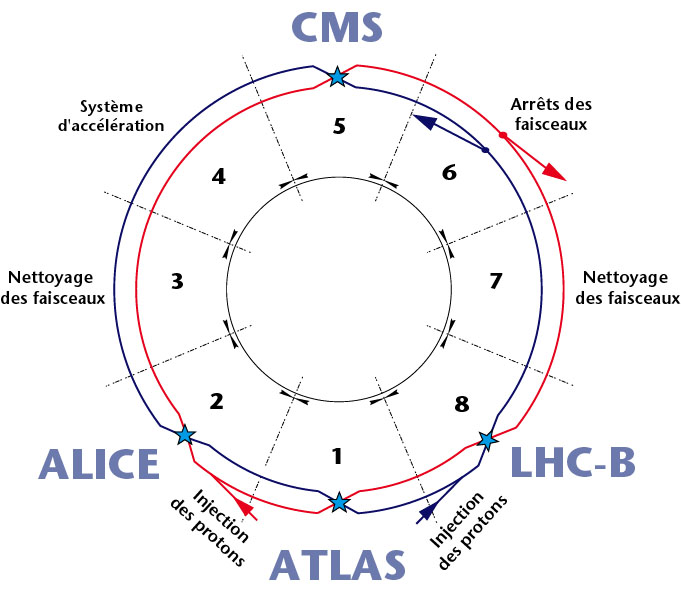
\includegraphics[width=0.55\textwidth]{LHC/lhc-schematic.jpg}
  	\captionof{figure}{Vue schématique des $8$ octants du LHC ainsi que des positions des principaux détecteurs le long du LHC. Les faisceaux (en bleu et rouge) circulent en sens inverse l'un de l'autre.}
  	\label{octants}	
  	\par 	
\marginpar
{
    \vspace*{-7.5cm}
	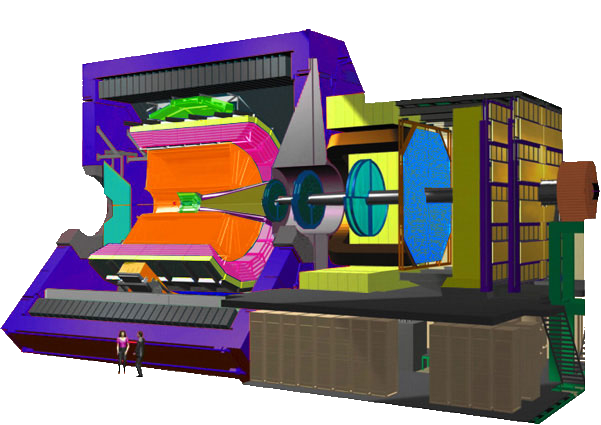
\includegraphics[width=\marginparwidth]{LHC/alice.png}
    \captionof{figure}{ALICE.}
    	\label{alice}
}
\end{minipagewithmarginpars}
\marginpar
{
	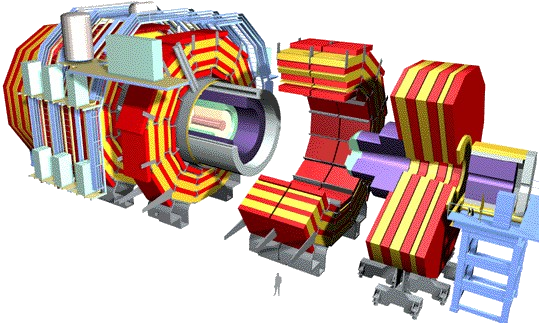
\includegraphics[width=\marginparwidth]{LHC/cms.png}
    \captionof{figure}{CMS.}
    	\label{cms}
}
\marginpar
{
	
	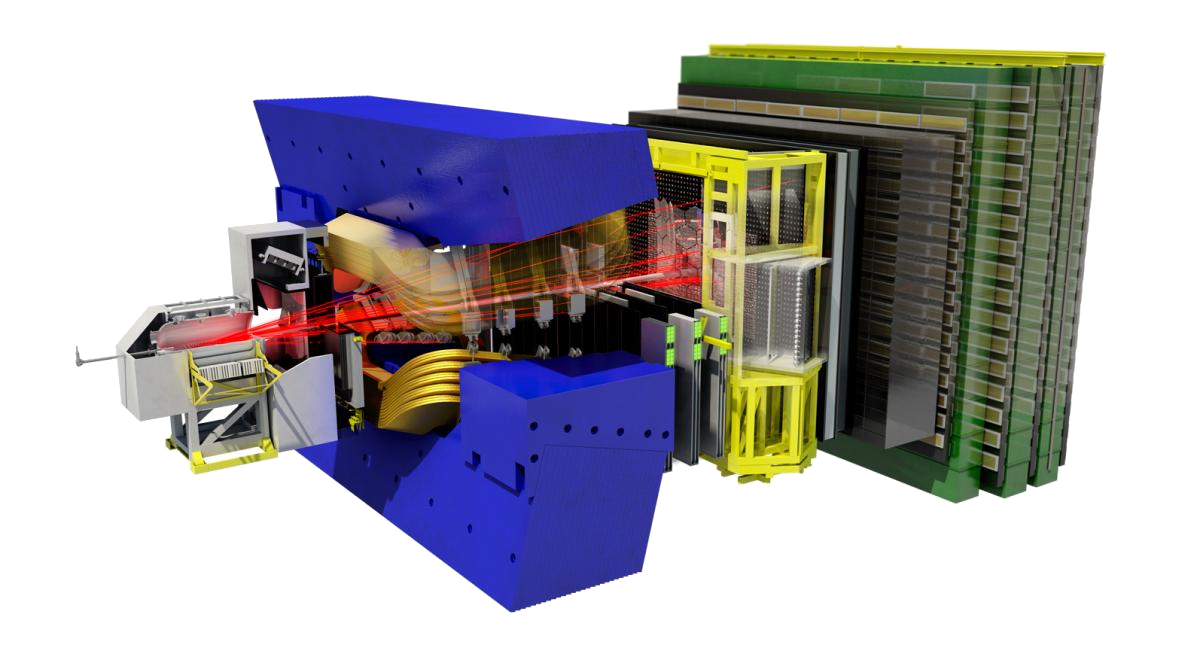
\includegraphics[width=\marginparwidth]{LHC/lhcb.png}
    \captionof{figure}{LHCb.}
    	\label{lhcb}
}